% !TEX root=../main.tex
\subsubsection{Problem Definition:}
Let $Y={y_1,\dots,y_s}$ and $Z={z_1,\dots,z_u}$ denote a set of $s$ seen and $u$ unseen group
labels, and they are disjoint $Y \cap Z = $\O$ $. Similarly $S_Y={s_1,\dots,s_s}$ $\in \mathcal{R}^{s \times k}$ and $S_Z={s_1,\dots,s_u}$ $\in \mathcal{R}^{u \times k}$ denote the corresponding seen and unseen class semantic
representations (e.g. k-dimensional attribute vector).

Given training data with N number of samples $X_Y={(xi; yi; si)}  \in R^{d \times N}$
,where $x_i$ is a $d$-dimensional $i$-th training image from
one of the seen groups, zero-shot learning (ZSL) aims to detect
anomalous groups of images $f : X_Z \longrightarrow Z$
from unseen test data comprising of either only $X_Z= {(xi; zu; su)}$ or $X_Y \cup X_Z $ in case of generalized zero shot learning setting wherein $z_u$ and $s_u$ are unknown.

\subsubsection{ Zero Shot Learning based Embedding with SAE : }
Following the remarkable success of representation learning and deep learning,  a framework of embedding with autoencoder regularization (EAER)~\cite{yu2013embedding}, which incorporates embedding and autoencoding techniques. The joint minimization of the embedding loss and the autoencoder reconstruction error ensures the autoencoder is trained with the input embedding constraints. Embedding constraints enable to include the meta information about inputs such as similarity of data points or group attributes. As shown in Equation~\ref{eqn:embedded-semantic-ae-modified} we aim to simultaneously minimize the autoencoder reconstruction error at the output layer and the embedding loss in the hidden layer.
\begin{equation}
  \label{eqn:embedded-semantic-ae-modified}
  \begin{aligned}
  \min_{\W} \| \X - \W^T \S ) \|_F^2  + \lambda \| \W\X - \S ) \|_F^2 + \beta \sum_{n=1}^{d} KL(\rho||\hat\rho_n) \\
  + \sum_{1\leq i\leq j \leq N} L(f(\W,\X_i),f(\W,\X_j),\varphi_{ij}) \\
\end{aligned}
\end{equation}


\begin{figure}[t]
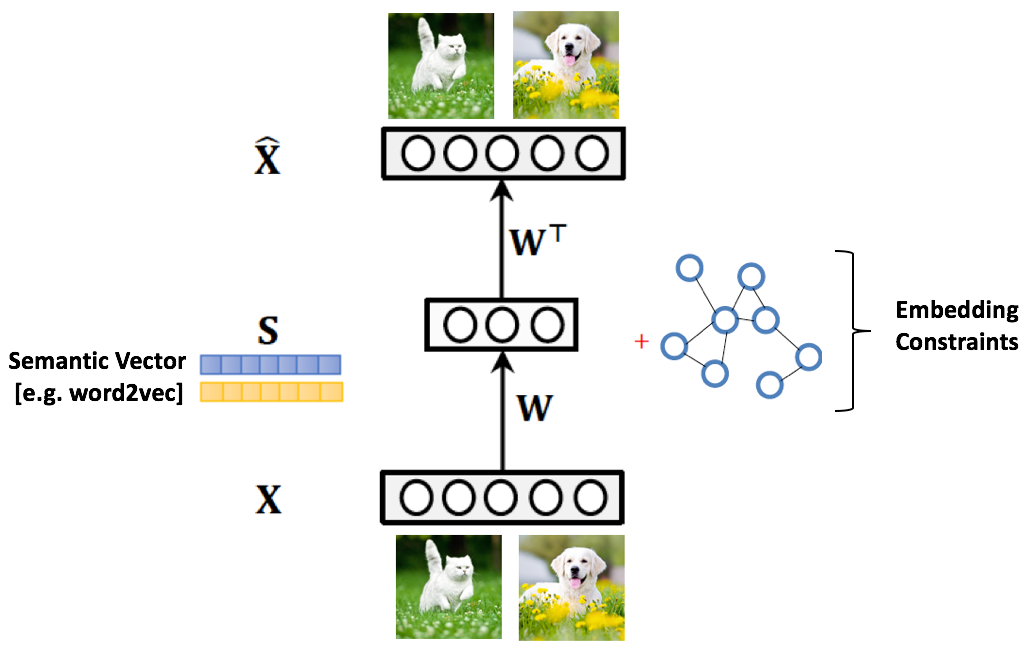
\includegraphics[scale=0.55]{images/SemanticAE_WithEmbeddingConstraints}
\centering
\caption{Zero shot learning (ZSL) based Semantic Autoencoder (SAE) with embedding constraints for group anomaly detection. }
\label{fig:ZSL_SAE_Embedding}
\end{figure}


Equation~\ref{eqn:embedded-semantic-ae-modified} is a joint objective of both semantic autoencoder loss and the embedding loss. $L(.)$ is the embedding loss function between pairs of the data (its detailed
form can be any of the functions described in Section~\ref{sec:laplacianEmbd}, Section~\ref{sec:msembedding} and Section~\ref{sec:MarginBasedEmbd} for various embedding al-
gorithms) that may be used as constraints. Here, $f(W,X_i),f(W,X_j)$ maps input data points $X_i,X_j$ to the low dimension latent representation. \\
$\beta$ is the sparsity penalty term  and $\lambda$ is weight decay term  used in autoencoder regularization. The regularization terms aid in embedding and facilitate towards better data representations of the group.
We consider sparse autoencoder with sparsity parameter $\rho$ and penalize it with the Kullback-Leibler (KL) divergence~\cite{hinton2012practical}. Where $\rho$ is a sparsity constraint parameter ranges from 0 to 1 and $\beta$ controls the sparsity penalty term. The $KL(\rho||\rho_n )$ attains a minimum value when $\rho = \rho_n$ , where $\rho_n$ denotes the average activation value of hidden unit $n$ over the all training inputs $X$.


\subsubsection{ Supervised clustering  for group anomaly detection: }
With the encoder projection matrix $\W$:  obtained after training the autoencoder with the proposed objective function as per Equation~\ref{eqn:embedded-semantic-ae-modified}. We can embed
a new test sample $xi \in X_Z$ to the semantic space by $si = \W x_i$.
The samples belonging to anomalous groups can be detected by simply calculating
the euclidean distance between the estimated semantic
representation $si$ and the prototypes of unseen group label set $S_Z$. The semantic representation $si$ closer to the unseen group label represent the anomalous group within the data instances. Using SAE embedded with group attribute constraints in a ZSL training mode uncovers the previously unknown group that may exist within the input data.

\begin{figure}[t]
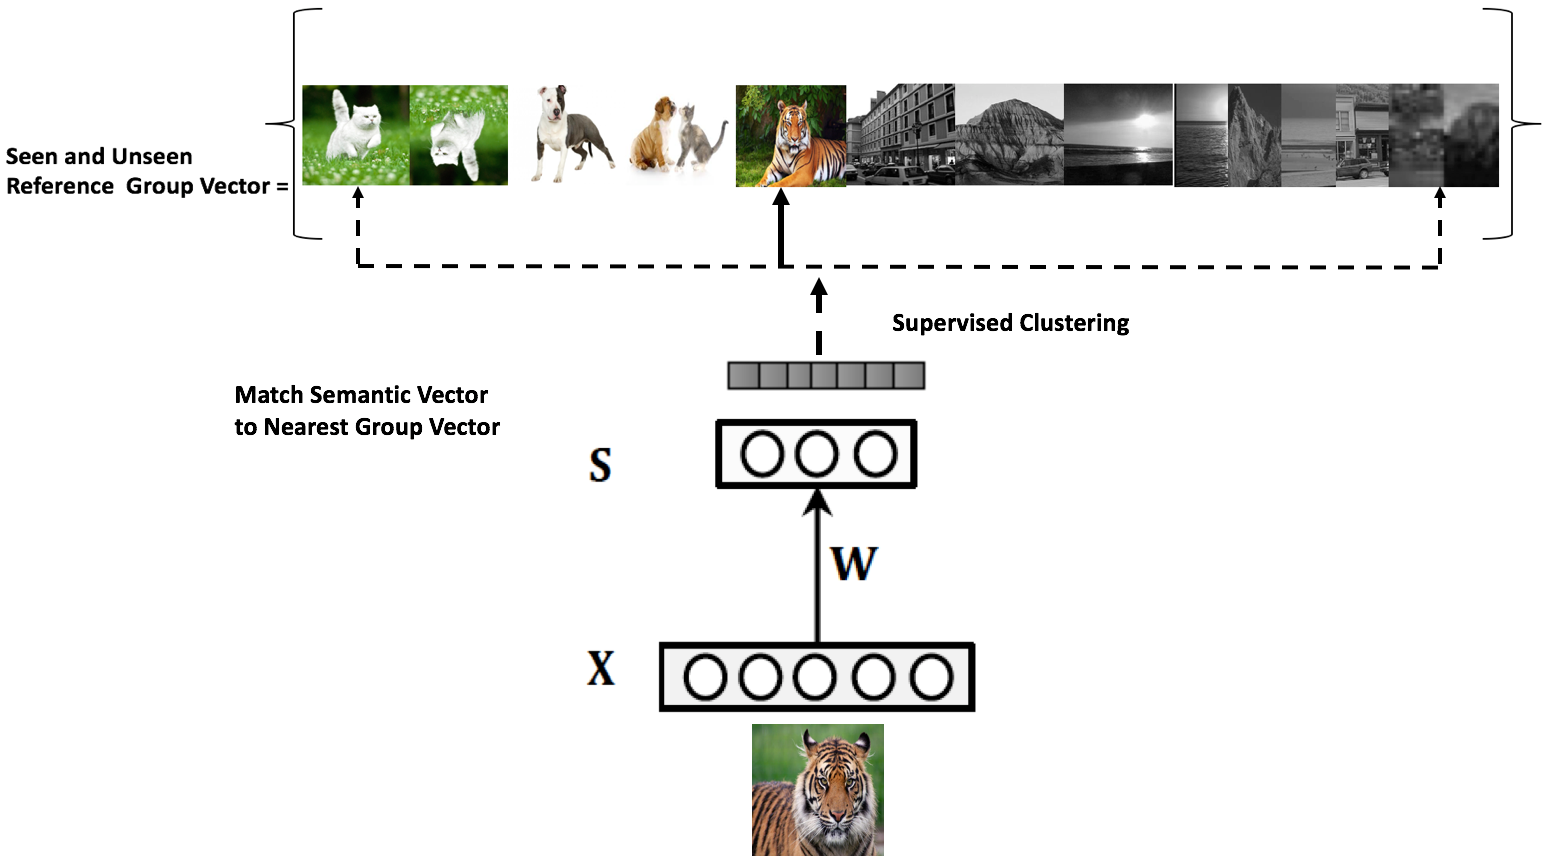
\includegraphics[scale=0.50]{images/encoderGrpEmbedding}
\centering
\caption{Supervised Clustering using on the ZSL semantic embeddings to detect group anomalies. }
\label{fig:encoderGrpEmbedding}
\end{figure}



% We now present our robust (convolutional) autoencoder model for anomaly detection.
% The method can be seen as an extension of robust PCA to allow for a nonlinear manifold that explains most of the data.
% %
% \subsection{Robust (convolutional) autoencoders}
% Let $f \colon \Real \to \Real$ be some non-decreasing {activation function}.
% Now consider the following objective, which combines the salient elements of Equations \ref{eqn:autoencoder} and \ref{eqn:robust-pca}:
% \begin{equation}
% 	\label{eqn:robust-ae}
% 	\min_{\U, \V, \N} \| \X - (f(\X \U) \V + \N) \|_F^2 + \frac{\mu}{2} \cdot (\| \U \|_F^2 + \| \V \|_F^2) + \lambda \cdot \| \N \|_1,
% \end{equation}
% where $f( \cdot )$ is understood to act elementwise, and $\lambda, \mu > 0$ are tuning parameters.
% This is a form of \emph{robust autoencoder}:
% one encodes the input into the latent representation $\Z = f( \X \U )$,
% which is then decoded via $\V$.
% The additional $\N$ term captures gross outliers in the data, as with robust PCA.
% For the purposes of anomaly detection, we have reconstruction matrix $\hat{\X} = f(\X \U) \V$.

% When $\lambda \to +\infty$, we get $\N = \mathbf{0}$, and the model reduces to a standard autoencoder (Equation \ref{eqn:autoencoder}).
% When $\lambda \to 0$, then one possible solution is $\N = \X$ and $\U = \V = \mathbf{0}$, so that the model memorises the training data.
% For intermediate $\lambda$, the model augments a standard autoencoder with a noise absorption term that endows robustness.

% More generally, Equation \ref{eqn:robust-ae} can be seen as an instance of
% \begin{equation}
% 	\label{eqn:robust-cae}
% 	\min_{\theta, \N} \| \X - (\hat{\X}( \theta ) + \N) \|_F^2 + \frac{\mu}{2} \cdot \mathrm{\Omega}( \theta ) + \lambda \cdot \| \N \|_1,
% \end{equation}
% where $\hat{\X}( \theta )$ is some generic predictor with parameters $\theta$, and $\mathrm{\Omega}( \cdot )$ a regularisation function.
% Observe that we could pick $\hat{\X}( \theta )$ to be a convolutional autoencoder~\cite{Jain:2008,vincent2010stacked}, which would be suitable when dealing with image data;
% such a model will be studied extensively in our experiments.
% Further, the regulariser $\mathrm{\Omega}$ could involve more general matrix norms, such as the $\ell_{1,2}$ norm \cite{Huang:2010}.


% %
% \subsection{Training the model}
% \label{sec:training}

% The objective function of the model of Equation \ref{eqn:robust-ae}, \ref{eqn:robust-cae} is non-convex, but unconstrained and sub-differentiable.
% There are several ways of performing optimisation.
% For example, for differentiable activation $f$, one could compute sub-gradients with respect to all model parameters and apply backpropagation.
% However, to leverage existing advances in training deep networks, we observe that:
% \begin{itemize}
% 	\item For fixed $\N$, the objective is equivalent to that of a standard (convolutional) autoencoder on the matrix $\X - \N$.
% 	Thus, one can optimise the parameters $\theta$ using any modern (stochastic) optimisation tool for deep learning that exploits gradients, such as Adam \cite{kingma2014adam}.

% 	\item For fixed $\theta$ (i.e.\, $\U, \V$ in the standard autoencoder case), the objective is
% 	$$ \min_{\theta, \N} \| \N - (\X - \hat{\X}( \theta )) \|_F^2 + \lambda \cdot \| \N \|_1, $$
% 	which trivially solvable via the soft thresholding operator on the matrix $\X - \hat{\X}( \theta )$ \cite{Bach:2011}, with solution
% 	$$ \N_{ij} =
% 	\begin{cases}
% 		(\X - \hat{\X}( \theta ))_{ij} - \frac{\lambda}{2} & \text{ if } (\X - \hat{\X}( \theta ))_{ij} > \frac{\lambda}{2} \\
% 		(\X - \hat{\X}( \theta ))_{ij} + \frac{\lambda}{2} & \text{ if } (\X - \hat{\X}( \theta ))_{ij} < -\frac{\lambda}{2} \\
% 		0 & \text{ else. }
% 	\end{cases}
% 	$$
% \end{itemize}
% We thus alternately optimise $\N$ and $\theta$ until the change in the overall objective is below some threshold.
% The use of stochastic optimisation for the first step, and the simplicity of the optimisation for the second step, means that we can easily train the model where data arrives in an online or streaming fashion.


% %
% \subsection{Predicting with the model}

% One convenient property of our model is that the anomaly detector will be inductive, i.e.\ it can generalise to unseen data points.
% One can interpret the model as learning a robust representation of the input, which is unaffected by gross noise;
% such a representation should thus be able to accurately model any unseen points that lie on the same manifold as the data used to train the model.

% Formally, given a new $\mathbf{x}_* \in \Real^D$, one simply computes $f( \mathbf{x}_*^T \U ) \V$ to score this point.
% The larger $\| \mathbf{x}_* - \V^T f( \U^T \mathbf{x}_* ) \|_2^2$ is, the more likely the point is deemed to be anomalous.
% We emphasise that such inductive predictions are simply not possible with the robust PCA method, as it estimates parameters for the $N \times D$ observations present in $\X$, with no means of generalising to unseen data.



% %
% \subsection{Connection to robust PCA}

% While the robust autoencoder of Equation \ref{eqn:robust-ae} has clear conceptual similarity to robust PCA,
% it may seem that choices such as the $\ell_2$ penalty on $\U, \V$ are somewhat arbitrarily used in place of the trace norm.
% We now show how the objective can in fact be naturally derived as an extension of OCSMM.

% The trace norm can be represented in the variational form~\cite{recht2010guaranteed}
% $ \| \S \|_* = \min_{\W \V = \S} \frac{1}{2} \cdot (\| \W \|_F^2 + \| \V \|_F^2). $
% The robust PCA objective is thus equivalently
% $$ \min_{\W, \V, \N} \frac{1}{2} \cdot (\| \W \|_F^2 + \| \V \|_F^2) + \lambda \cdot \| \N \|_1 : \X = \W \V + \N. $$
% This objective has the disadvantage of being non-convex,
% but the advantage of being amenable to extensions.
% Pick some $\mu > 0$, and consider a relaxed version of the robust PCA objective:
% $$ \min_{\W, \V, \N, \E} \| \E \|_F^2 + \frac{\mu}{2} \cdot (\| \W \|_F^2 + \| \V \|_F^2) + \lambda \cdot \| \N \|_1 : \X = \W \V + \N + \E. $$
% Here, we allow for further systematic errors $\E$
% which have low average magnitude.
% We can equally consider the unconstrained objective
% \begin{equation}
% 	\label{eqn:rpca-v2}
% 	\min_{\W, \V, \N} \| \X - (\W \V + \N) \|_F^2 + \frac{\mu}{2} \cdot (\| \W \|_F^2 + \| \V \|_F^2) + \lambda \cdot \| \N \|_1
% \end{equation}
% This re-expression of robust PCA has been previously noted, for example in Sprechmann et al.~\cite{Sprechmann:2015}.
% To derive the robust autoencoder from Equation \ref{eqn:rpca-v2}, suppose now that we constrain $\W = \X \U$.
% This is a natural constraint in light of Equation \ref{eqn:pca}, since for standard PCA we factorise $\X$ into $\hat{\X} = \X \U \U^T$.
% Then, we have the objective
% $$ \min_{\U, \V, \N} \| \X - (\X \U \V + \N) \|_F^2 + \frac{\mu}{2} \cdot (\| \X \U \|_F^2 + \| \V \|_F^2) + \lambda \cdot \| \N \|_1. $$
% Now suppose we modify the regulariser to only operate on $\U$ rather than $\X \U$:
% $$ \min_{\U, \V, \N} \| \X - (\X \U \V + \N) \|_F^2 + \frac{\mu}{2} \cdot (\| \U \|_F^2 + \| \V \|_F^2) + \lambda \cdot \| \N \|_1. $$
% This is again natural in the context of standard PCA, since there we have $\W = \X \U$ satisfying $\W^T \W = \I$.
% Observe now that we have derived Equation \ref{eqn:robust-ae} for a linear activation function $f( x ) = x$.
% The robust autoencoder thus extends this model by employing a nonlinear activation.


% %
% \subsection{Relation to existing models}

% Our contribution is a nonlinear extension of OCSMM for anomaly detection.
% As noted above, the key advantages over OCSMM are the ability to capture nonlinear structure in the data, as well as the ability to detect anomalies in an inductive setting.
% The price we have to pay is the lack of convexity of the objective function, unlike OCSMM;
% nonetheless, we shall demonstrate that the model can be effectively trained using the procedure described in Section \ref{sec:training}.

% Some works have employed deep networks for anomaly detection~\cite{Williams:2002,Zhai:2016},
% but without explicitly accounting for gross anomalies.
% For example, the recent work of \cite{Zhai:2016} employed an autoencoder-inspired objective to train a probabilistic neural network, with extensions to structured data;
% the use of an OCSMM-style noise matrix $\N$ may be useful to explore in conjunction with such methods.

% Our method is also distinct to denoising autoencoders (DNA), wherein noise is explicitly added to instances~\cite{vincent2010stacked}, whereas we \emph{infer} the noise automatically.
% The approaches have slightly different goals: DNAs aim to extract good features from the data, while our aim is to identify anomalies.

% Finally, while nonlinear extensions of PCA-style matrix factorisation (including via autoencoders) have been explored in contexts such as collaborative filtering \cite{Lawrence:2009,Sedhain:2015}, we are unaware of prior usage for anomaly detection.
